%
% methods_data_transmission.tex
%

Our client-side architecture consists of one primary abstraction for chart components.  By abstracting chart components behind a common interface, we can accomplish charting platform agnosticism and create a predictable life cycle governing the loading of datasets and rendering of charts.  Our client, much like the server, has a “driver” component.  The driver component should be static as the architecture seeks to encapsulate all common avenues of change within the chart components.  The driver’s goal is to handle server-client communications and enable the user to query data as the developer sees appropriate.  The driver can simply load a default query from the server or include a query builder for the client’s use.  The developer can choose which functionality best suits their needs, but the application should utilize the common chart component interface to interact with charts. \par
The client-side design and implementation are quite simple. The following sections will overview each feature, discuss the architectural decisions, and present our implementation.  The client-side architecture draws more direct inspiration from Angular’s component system, however it is easily implementable across different client-side frameworks or even in framework-less client-side code. \par

\subsection{Chart Components}
Our primary client-side abstraction defines a common interface for charts.  Each chart component should define a single renderable chart, although the developer can freely define multiple charts, widgets, or other data visualization features within a single component.  A“single component - single chart” policy is recommended to improve modularity but it is not strictly enforced.  Each charting component must implement a common interface, visualized in Figure 5.4.1 as the \textit{ChartComponent} interface. This interface requires the charting component to have a list of required datasets, a function to access that list, and a function to update the chart’s data.  This interface allows the charting components to be loosely coupled with the driver.  Once the driver has received data, it obtains a list of a chart component’s required datasets, validates that it can provide all the required datasets, and calls that components lifecycle hook to update it (\textit{updateChart} in \ref{fig:client-side-class}). \par
By interacting with charting components only through a common interface, we eliminate any coupling between data acquisition control logic and chart rendering.  Our architecture is reminiscent of an observer pattern.  The client driver will serve only one primary purpose: to query data from the server and ingest that data.  Once it has obtained that data, it “notifies” the chart components of updated data using their \textit{updateChart} lifecycle hook.  The chart components, in this instance, are our observers, waiting for changes from the driver.  This system allows the developer to define data acquisition code in the driver once, and modularly add charting components.  This also introduces the possibility of dynamic chart components that allow the user to select what data is shown/compared within the chart component. \par
Chart components also allow the data acquisition “business logic” to be entirely independent and unaware of the charting libraries in use.  This allows our architecture to provide complete charting platform agnosticism.  The developer can change charting libraries by simply writing new charting components that utilize a new library.  A single client page can even include multiple charts from multiple charting libraries, all encapsulated within their own chart components.  All of this can be achieved with no change to the data acquisition/business logic in the driver. \par
Beestream’s client is implemented using Angular as a client-side framework.  Angular’s framework includes constructs for modules and components to define functionality and pages. Angular also utilizes Typescript which provides class and inheritance constructs.  This allows us to implement the client-side architecture shown in Figure \ref{fig:client-side-class} almost directly.  The implementation includes a single module for the charting page, which declares a single driver component and all registered chart components.  The driver has knowledge of all chart components as part of its renderable template.  The driver holds all server-client interaction logic and includes a small widget to allow the user to build simple queries.  Angular renders pages by calling a series of lifecycle hooks.  These lifecycle hooks are also intercepted by the driver.  Once the page is initialized, as is signaled by the \textit{afterViewInit} lifecycle hook, chart components are rendered.  These charting components can determine their own behavior after initial rendering, although in our case they simple render as hidden.  Each chart component is implemented as a separate Angular component that implements a ChartComponent interface.  As such, the driver is guaranteed to have access to a method to update the chart and a method to list required datasets.  Overall, our implementation maps almost directly to the defined architecture. \par

\begin{figure}
  \centering
  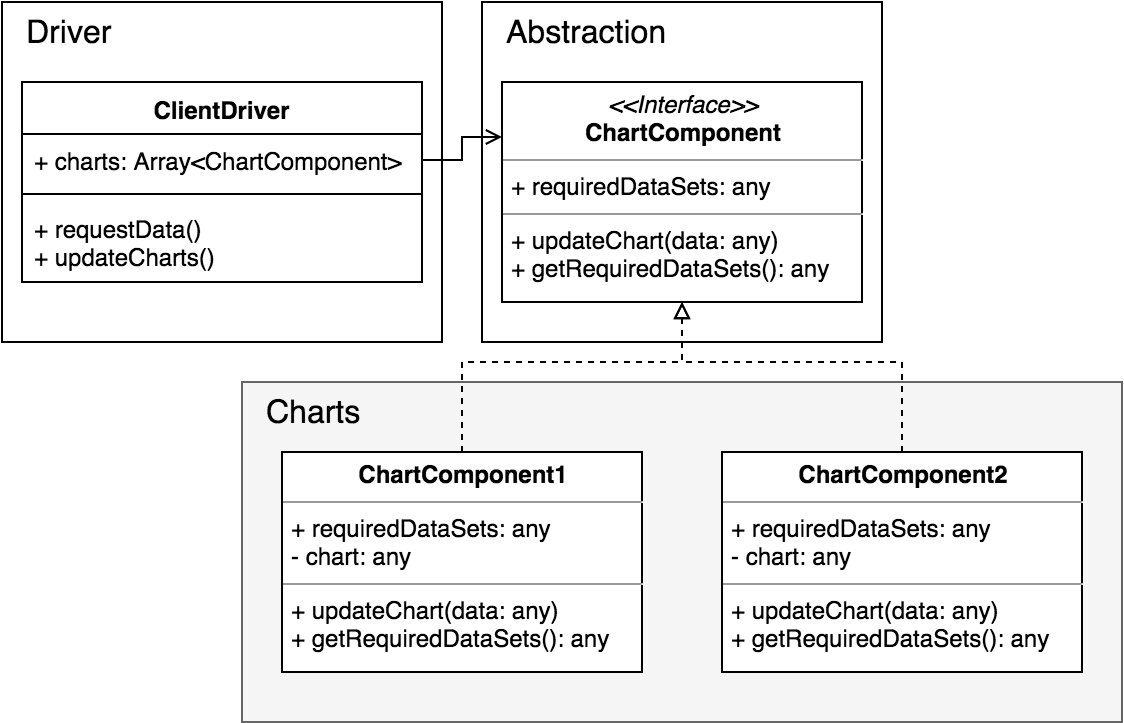
\includegraphics[width=6in]{images/ClientSide.png}
  \caption{Client Side Class Diagram}
  \label{fig:client-side-class}
\end{figure}

\subsection{Dataset Request Flow}

Our architecture presents a simple dataset request flow which allows each charting component to request datasets.  Each chart will only be updated and rendered if the required datasets are available.  This offers the guarantee that empty charts will not be rendered if data is missing, avoiding any errors associated with rendering an empty chart.  This behavior is enforced by using the simple handshake shown in Figure \ref{fig:client-dataset-request} before any data request is made and the handshake shown in Figure \ref{fig:client-update-flow} after data is received.  These handshakes must be enforced by the developer-defined client driver.  Using these handshakes, the driver can ensure that it queires only the necessary datasets from the server to reduce data transmission size and render only those charts whose data is available. \par
\begin{figure}
  \centering
  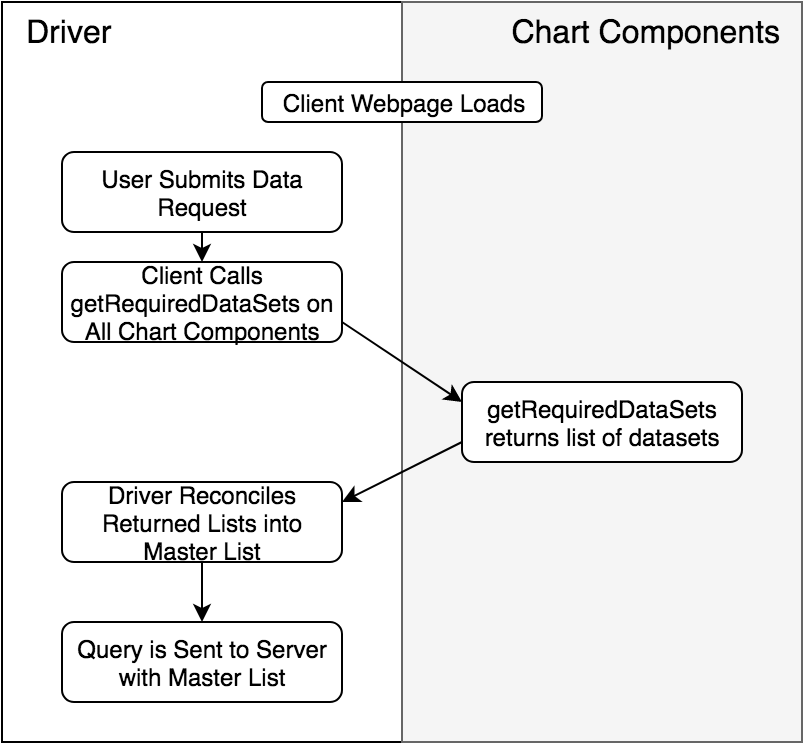
\includegraphics[width=4in]{images/ClientDatasetRequestFlow.png}
  \caption{Client Dataset Request Flowchart}
  \label{fig:client-dataset-request}
\end{figure}

\begin{figure}
   \centering
   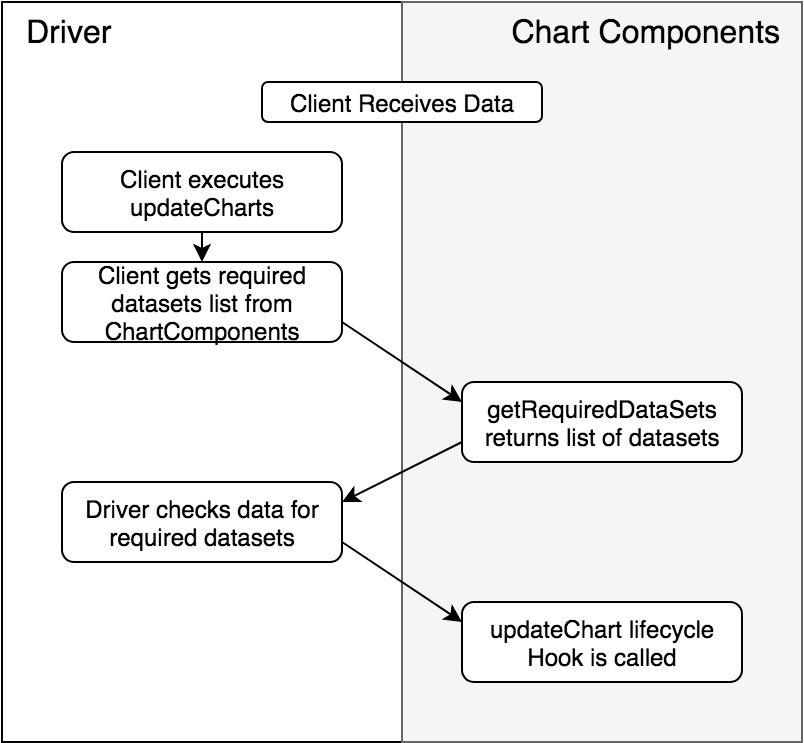
\includegraphics[width=4in]{images/ClientChartUpdateFlow.png}
   \caption{Client Chart Update Flowchart}
   \label{fig:client-update-flow}
\end{figure}

The first handshake occurs after rendering the page, rendering chart components, and only after the driver has received the initial list of available datasets from the server.  Before the client driver sends a data request to the server, it will poll every chart component for its required datasets.  Using this information, the client driver will populate a list of all unique required datasets.  This list should be cross-checked with the list of available datasets sent from the server.  After any unavailable datasets are removed from the list, it will be used as a parameter in the data request.  This step ensures that the client requests only the data it needs to render charts, avoiding unnecessary data transmission. \par
The second handshake occurs when the client driver receives data back from the client after issuing a data request.  In this handshake, the driver will iterate through all chart components.  The driver will check each chart component’s required datasets list and, if all dataset needs are met, it will call that component’s update lifecycle hook and pass it the relevant updated data.  If all required datasets are not available, the update hook will not be called.  If the developer desires, they can add a “missing data” lifecycle hook to the chart component interface and call this hook if required datasets are not present.  This handshake ensures that charts are only rendered if all required data is present. \par

\subsection{Lifecycle Control}

In sections 5.4.1 and 5.4.2, we’ve frequently referenced a chart “lifecycle.”  Our architecture defines a certain lifecycle for rendered chart components through both implicit driver logic and the chart component interface.  The client driver ultimately controls when and how charts are rendered and delivered data.  As such, the driver controls the lifecycle of the chart components.  As discussed in section 5.4.2, each chart is only rendered and updated with data if the required data is available.  These extra steps can be seen in figure \ref{fig:client-lifecycle-flow}.  The handshakes discussed in 5.4.2 define a simple lifecycle for a chart, however our driver can more strictly enforce a lifecycle through the use of Angular’s lifecycle hooks. \par
\begin{figure}
    \centering
    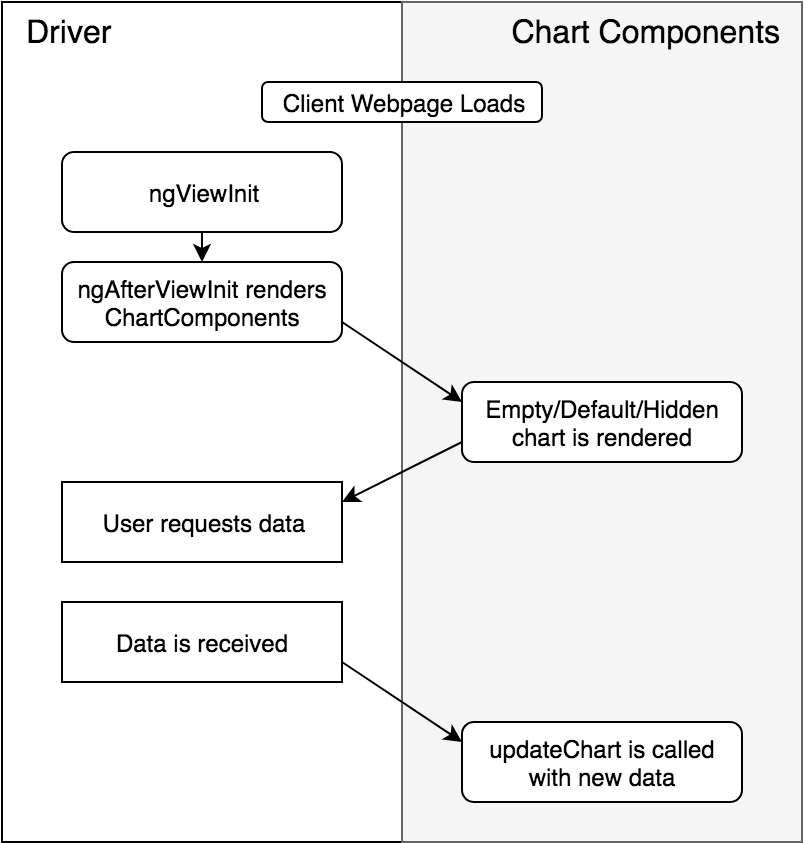
\includegraphics[width=4in]{images/ClientLifecycle.png}
    \caption{Client Chart Lifecycle Flowchart}
    \label{fig:client-lifecycle-flow}
\end{figure}
Depending on the charting library, charts can be dynamically generated, populated, updated, and destroyed.  In Beestream’s implementation, C3.js charts are utilized.  In this library, charts are bound to a single HTML element after the page is fully rendered.  As such, each chart component shouldn’t be rendered until after the webpage is rendered.  This is enforced by having each chart component using C3.js implement the \textit{ngAfterViewInit} lifecycle hook.  The chart can render at this time, but it doesn’t need to be shown yet because it hasn’t been given data.  The client driver is responsible for handling this part of the lifecycle.  As a result, Beestream’s chart components must respect Angular’s lifecycle for chart rendering and the client driver’s lifecycle for chart display and population.  The chart is “rendered” but hidden until the client driver allows it to populate. \par
